\documentclass{article}
\usepackage{iclr2027_conference,times}
\input{math_commands.tex}

\usepackage{amsmath,amsfonts,amssymb}
\usepackage{array}
\usepackage{booktabs}
\usepackage{graphicx}
\usepackage{float}
\usepackage{algorithm}
\usepackage{algorithmic}
\usepackage{hyperref}
\hypersetup{hidelinks}
\usepackage{url}

\newcommand{\up}{\ensuremath{\uparrow}}
\newcommand{\down}{\ensuremath{\downarrow}}
\newcommand{\algcall}[2]{\mathrm{#1}(#2)}

\title{Semantic Contracts for Traceable NL-to-Code Generation}
\author{Anonymous Authors}

% Uncomment only for the camera-ready version.
% \iclrfinalcopy

\begin{document}
\maketitle

\begin{abstract}
Large language models can generate code from natural-language problem statements, yet remain unreliable on constraint-intensive tasks. Failures may arise because a model misinterprets task semantics or because it implements a reasonable interpretation incorrectly. Requirement-alignment methods mainly improve task understanding before code generation, whereas program-repair methods use post-generation feedback to correct implementation errors. Their outputs, however, are rarely connected through an explicit and stable semantic target, leaving repair without consistent task-obligation constraints. We introduce a semantic-contract-based dual-loop framework that maintains the semantic target and program implementation as connected but independently managed states. The Semantic Alignment Loop (SAL) induces a structured specification, applies gated field-level revisions using a coverage--faithfulness--precision diagnostic profile and a Spec Alignment Score (SAS), and freezes the current specification at termination as a semantic contract. The Implementation Repair Loop (IRL) selects an initial program under that contract and performs iterative repair using public-test feedback and conservatively compiled property-clause feedback. This design records semantic revisions and implementation repairs as separate state transitions. On 1,055 LiveCodeBench release\_v6 problems, Full Dual-Loop produces 401 complete-suite passes, yielding a Final Pass Rate of 0.3801, 9.19 percentage points above Direct NL-to-Code and 3.98 points above the strongest shared-protocol external baseline. The results show improved final correctness while preserving inspectable evidence of task obligations and implementation transitions.
\end{abstract}

\section{Introduction}

Large language models have made natural-language-to-code generation a central problem in machine learning and software engineering. A natural-language task specifies input assumptions, output protocols, constraints, exceptional cases, and semantic conditions; a generated program is an executable implementation of those obligations. Existing systems improve reliability before generation through plans, pseudocode, retrieval, and requirement alignment \citep{ref_self_planning,ref_planning_driven_programming,ref_pseudocode_prompting,ref_codet,ref_acecoder,ref_mufix,ref_specfix,ref_reacoder}, or after generation through self-feedback, execution, compiler signals, and tests \citep{ref_self_refine,ref_reflexion,ref_opencodeinterpreter,ref_compiler_feedback,ref_stepcoder}.

Task misunderstanding and implementation error nevertheless remain distinct failure sources. Empirical studies report semantic misinterpretations, omitted requirements, and missing boundary cases that cannot be reduced to local coding mistakes \citep{ref_bug_study,ref_codegen_error_taxonomy,ref_nl_spec_verification_failure}. Requirement alignment and program repair usually operate as separate stages: the alignment result is not maintained as an explicit, stable target during repair, while repeatedly revising that target from execution failures makes task interpretation and implementation change together. In either case, repair lacks a consistent set of obligations against which successive programs can be compared.

We address this problem with a semantic-contract-based dual-loop framework that places an explicit state boundary between semantic alignment and implementation repair. SAL induces, diagnoses, and revises a structured specification. A candidate specification replaces the current state only after passing an acceptance gate; when SAL terminates, the current specification is frozen as the semantic contract. IRL then changes only program state: initial candidate selection and every repair round use the same contract. This boundary makes semantic revisions and implementation transitions separately observable.

Concretely, SAL represents task obligations in six field groups and uses a coverage--faithfulness--precision profile together with SAS to localize revisions. Safety and improvement predicates determine whether a field-level patch replaces the current specification. IRL generates an initial candidate set from the problem and frozen contract, selects one program using public feedback, and repairs only that current program over subsequent rounds. Verifier feedback is complemented by executable property clauses conservatively compiled from the contract, while private tests remain held out until final evaluation.

The main contributions are:
\begin{itemize}
    \item We formulate NL-to-code generation as two explicitly controlled state processes: SAL updates semantic state and freezes its accepted form before IRL updates implementation state.
    \item We develop a contract-conditioned mechanism that combines gated field-level revision, conservative property compilation, public-feedback-based initial selection, iterative repair, and an evidence-linked trace.
    \item We evaluate the framework on all 1,055 LiveCodeBench release\_v6 problems, three backbones, and 162 compatible HumanEval+ tasks, observing a 3.98-point gain over the strongest shared-protocol external baseline on the full release.
\end{itemize}

\section{Related Work}

\subsection{Intermediate representations}
Planning and pseudocode methods separate solution organization from implementation \citep{ref_self_planning,ref_pseudocode_prompting}. LPW generates a solution plan, verifies it on visible tests, and reuses the verified plan during code refinement \citep{ref_planning_driven_programming}. CodeT and AceCoder use generated tests or auxiliary artifacts to rank and refine candidates \citep{ref_codet,ref_acecoder}, while NL in the Middle studies natural-language intermediates for code translation \citep{ref_nl_middle}. These representations primarily describe how to solve or translate a task. Our specification instead records what every implementation must satisfy and remains available across candidate programs.

\subsection{Requirement alignment and multi-stage generation}
MuFix treats specification misunderstanding as a distinct pre-generation failure and repairs it using generated tests \citep{ref_mufix}. SpecFix detects ambiguous problem descriptions from behavioral clusters of generated programs and repairs the description through contrastive specification inference \citep{ref_specfix}. REA-Coder builds requirement-oriented questions and reference answers, then masks and recovers requirement fragments after generation; detected mismatches can return the system to requirement alignment \citep{ref_reacoder}. AlphaCodium and MapCoder organize problem analysis, planning, implementation, and debugging into multi-stage or multi-agent workflows \citep{ref_alphacodium,ref_mapcoder}. Our distinction is the lifecycle of the accepted requirement representation: SAL finishes before IRL, and execution feedback thereafter changes programs without reopening the semantic contract.

\subsection{Execution-guided repair and semantic failure analysis}
Self-Refine and Reflexion use model feedback or verbalized experience to guide iterative revision \citep{ref_self_refine,ref_reflexion}; OpenCodeInterpreter, COMPCODER, and StepCoder incorporate execution, compiler, or unit-test signals \citep{ref_opencodeinterpreter,ref_compiler_feedback,ref_stepcoder}. Complementary analyses show that generated code frequently omits constraints, invents assumptions, or mishandles edge cases, and that models struggle to verify code against natural-language specifications \citep{ref_bug_study,ref_codegen_error_taxonomy,ref_nl_spec_verification_failure}. These observations motivate an explicit semantic state that remains separate from executable implementation feedback.

\begin{figure}[t]
\centering
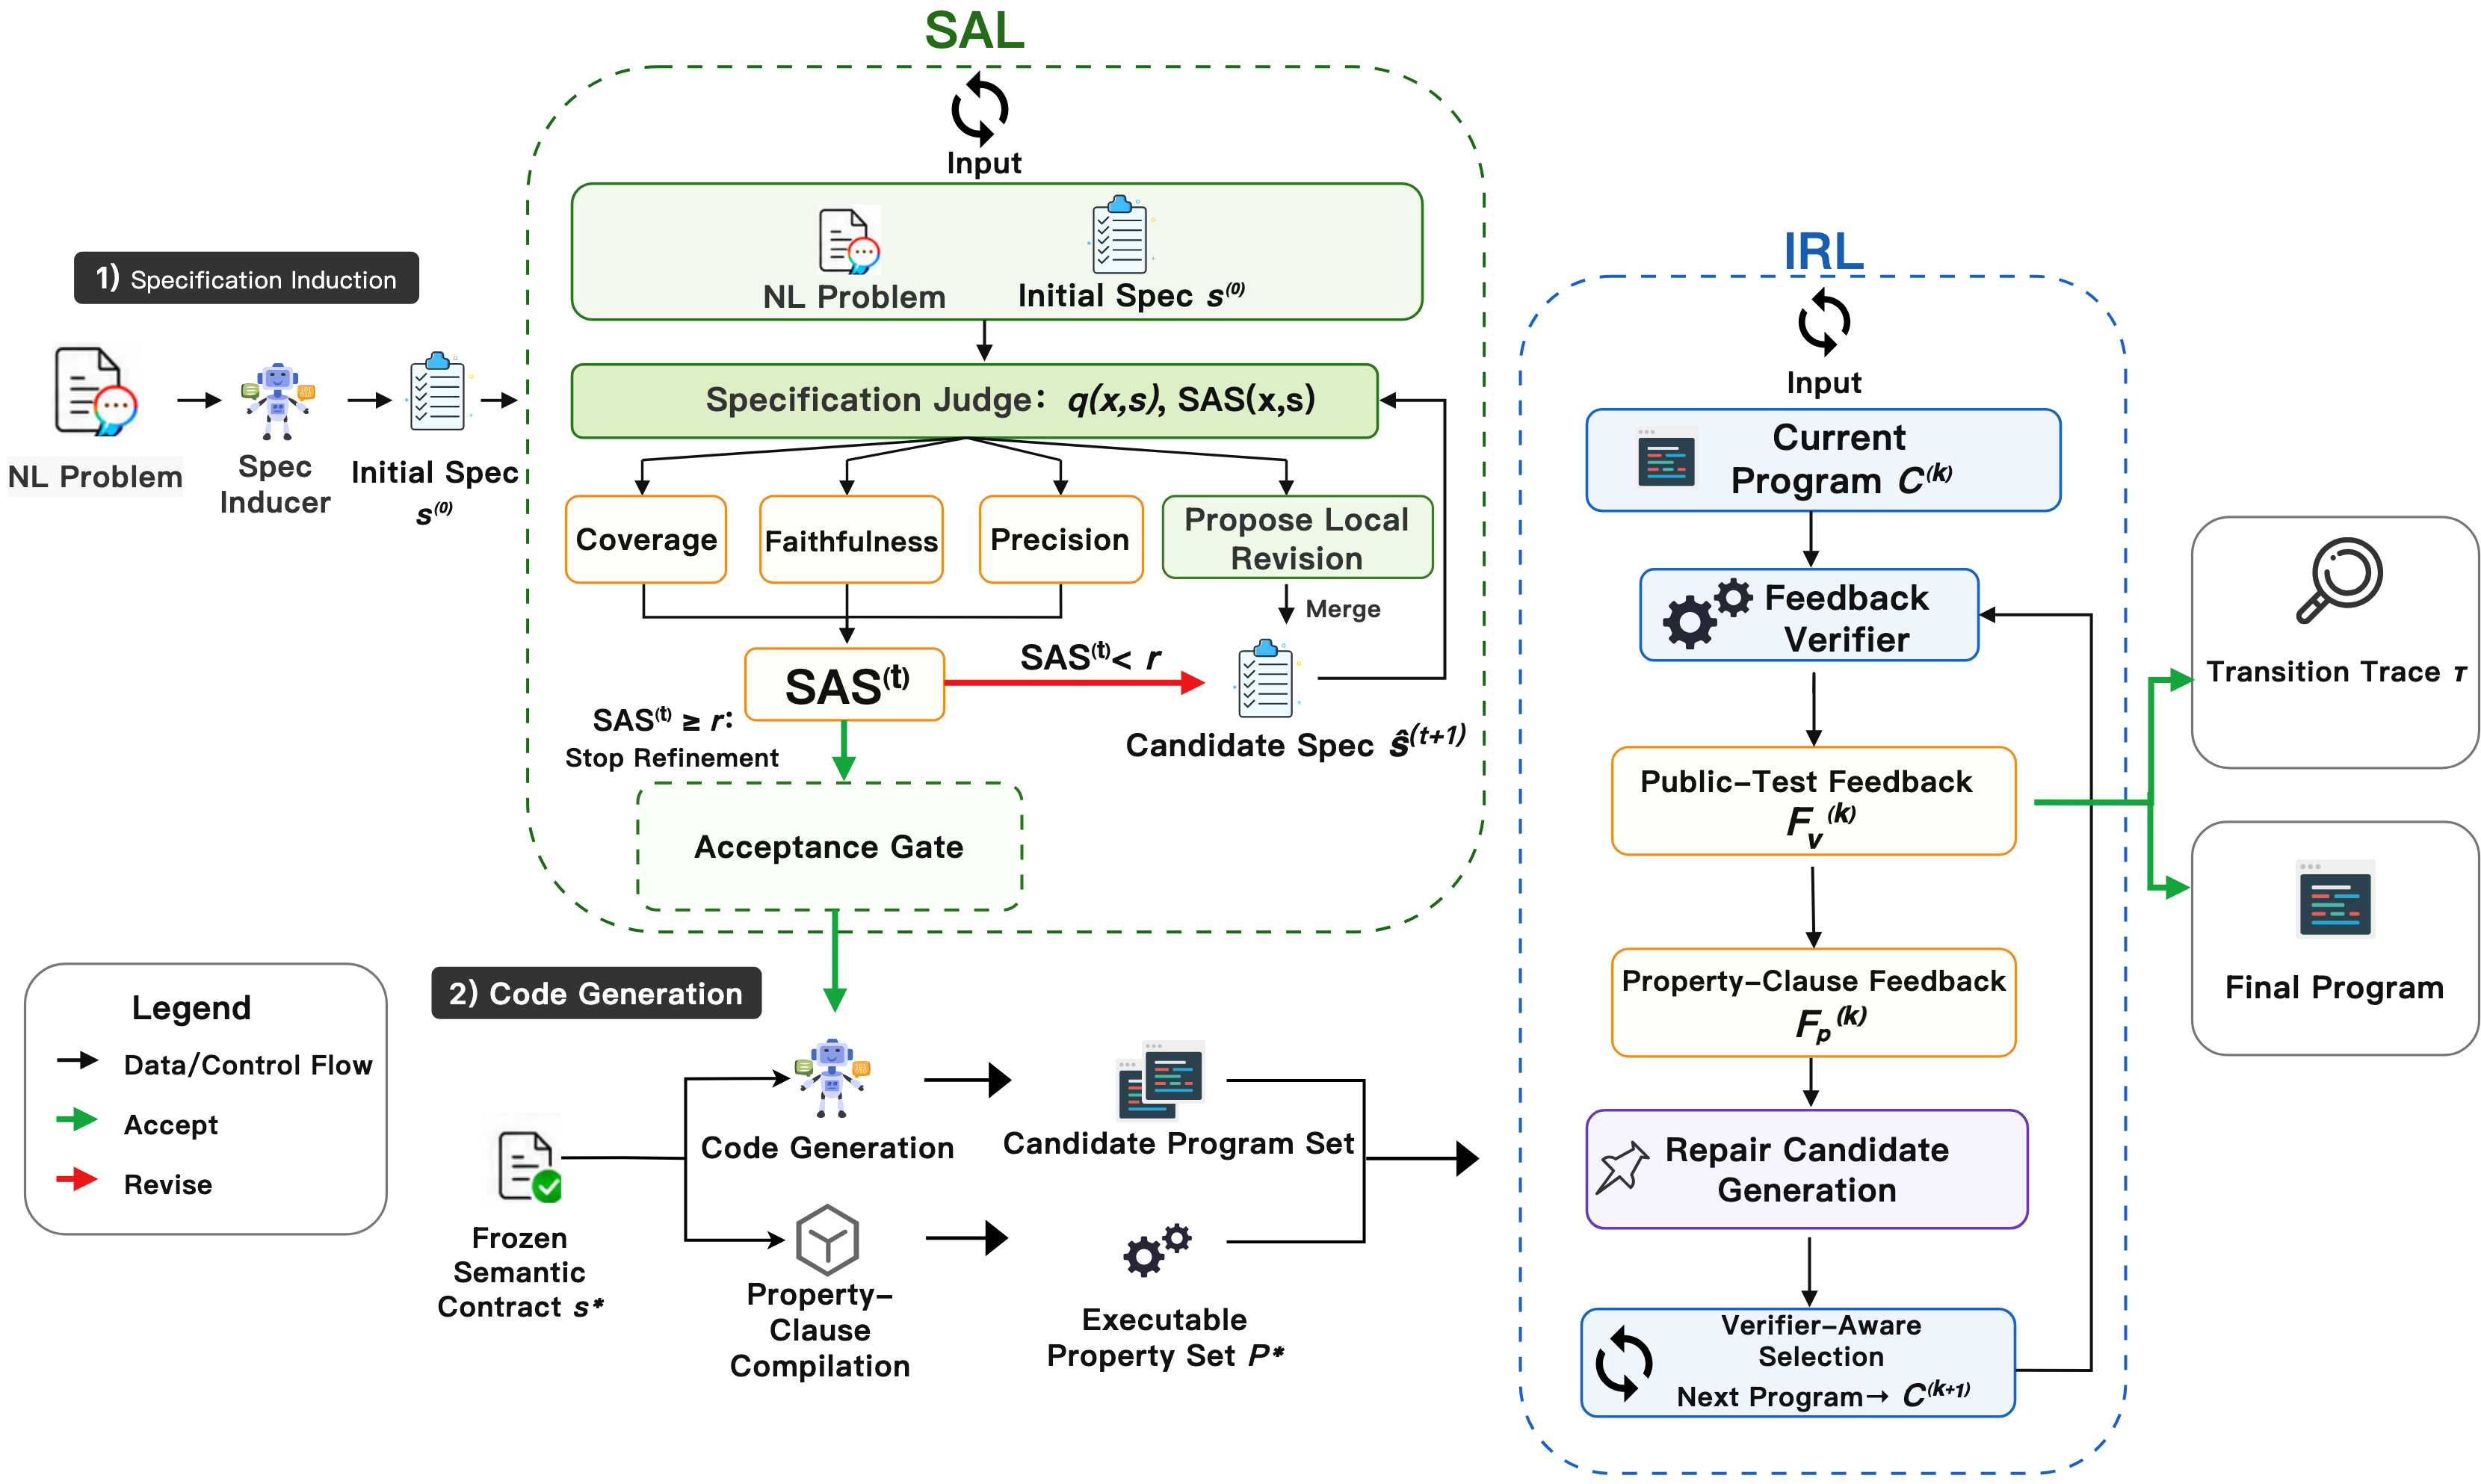
\includegraphics[width=\linewidth]{pics/framework_cn.png}
\caption{Overview of the dual-loop framework.}
\label{fig:framework}
\end{figure}

\section{Method}
The method is motivated by a state-observability problem. An incorrect program may follow from an inadequate task interpretation, an incorrect implementation of an adequate interpretation, or both. Direct NL-to-Code exposes only the final program and cannot show where the failure entered. We therefore place an explicit semantic state between problem $x$ and program $C$, revise that state before implementation, and hold it fixed during program repair.

\subsection{Overview}

Figure~\ref{fig:framework} divides generation into two connected stages. SAL induces an initial specification $s^{(0)}$. At semantic iteration $t$, it proposes a field-level patch $\Delta^{(t)}$, merges the patch with the current specification to obtain $\hat{s}^{(t+1)}$, and accepts the candidate only if it satisfies both safety and improvement conditions. An accepted candidate directly replaces the current state; a rejected candidate leaves $s^{(t)}$ unchanged and stops SAL. The current specification at termination is frozen as semantic contract $s^\star$, from which executable property set $P^\star$ is compiled.

IRL then generates an initial candidate set $\mathcal C^{(0)}$ from $(x,s^\star)$ and uses public feedback to select the unique initial state $C^{(0)}$. At round $k$, only current program $C^{(k)}$ is verified and repaired. The resulting repair candidates form the round-specific set $\mathcal C^{(k+1)}$, from which the system selects $C^{(k+1)}$. Unselected candidates from earlier rounds do not carry over. The complete process records semantic states, implementation states, and their evidence in trace $\tau$:
\begin{equation}
\begin{aligned}
x &\rightarrow s^{(0)}\rightarrow(q^{(0)},\mathrm{SAS}^{(0)})\rightarrow\cdots
\rightarrow(\Delta^{(t)},\hat{s}^{(t+1)})\\
&\rightarrow \mathrm{Accept}^{(t+1)}\rightarrow s^{(t+1)}\rightarrow\cdots
\rightarrow s^\star\rightarrow P^\star,\\
(x,s^\star)&\rightarrow\mathcal C^{(0)}\rightarrow C^{(0)}\rightarrow\cdots\rightarrow C^{(k)}\\
&\rightarrow(F_v^{(k)},F_p^{(k)})\rightarrow\mathcal C^{(k+1)}
\rightarrow C^{(k+1)}\rightarrow\cdots\rightarrow\tau.
\end{aligned}
\label{eq:transition}
\end{equation}
This boundary does not treat $s^\star$ as a proof of task intent. The contract is an LLM-induced, inspectable target; SAS is a directional evaluation signal; and only a limited subset of obligations can be compiled into executable clauses. Algorithm~\ref{alg:dual_loop} gives the complete control flow.

\begin{algorithm}[t]
\caption{Semantic-contract-based dual-loop generation}
\label{alg:dual_loop}
\begin{algorithmic}[1]
\REQUIRE problem $x$; SAL budget $T_s$; IRL budget $T_r$
\ENSURE final program $C$ and trace $\tau$
\STATE \textbf{Stage 1: semantic alignment}
\STATE $s^{(0)}\gets\algcall{InduceSpec}{x}$
\STATE $(q^{(0)},\mathrm{SAS}^{(0)})\gets\algcall{Judge_{\mathbf w}}{x,s^{(0)}}$
\FOR{$t=0,\ldots,T_s-1$}
  \IF{$\neg\algcall{ShouldRefine}{s^{(t)},q^{(t)},\mathrm{SAS}^{(t)},r}$}
    \STATE \textbf{break}
  \ENDIF
  \STATE $\Delta^{(t)}\gets\algcall{ProposePatch}{x,s^{(t)},q^{(t)}}$
  \STATE $\hat{s}^{(t+1)}\gets\algcall{Merge}{s^{(t)},\Delta^{(t)}}$; judge candidate
  \IF{$\mathrm{Safe}^{(t+1)}\land\mathrm{Improve}^{(t+1)}$}
    \STATE $s^{(t+1)}\gets\hat{s}^{(t+1)}$
  \ELSE
    \STATE $s^{(t+1)}\gets s^{(t)}$; \textbf{break}
  \ENDIF
\ENDFOR
\STATE $s^\star\gets$ current specification at SAL termination; freeze $s^\star$
\STATE $P^\star\gets\algcall{CompileClauses}{s^\star}$; initialize trace $\tau$
\STATE \textbf{Stage 2: implementation and repair}
\STATE $\mathcal C^{(0)}\gets\algcall{GenerateCandidates}{x,s^\star,N_0}$
\STATE $C^{(0)}\gets\algcall{SelectByFeedback}{\mathcal C^{(0)},x,s^\star,P^\star}$
\FOR{$k=0,\ldots,T_r$}
  \STATE $F_v^{(k)}\gets\algcall{Verify_{fb}}{x,C^{(k)}}$
  \IF{$\algcall{Pass}{F_v^{(k)}}\lor k=T_r$}
    \STATE \textbf{return} $(C^{(k)},\tau)$
  \ENDIF
  \STATE $F_p^{(k)}\gets\algcall{EvaluateClauses}{P^\star,x,C^{(k)},F_v^{(k)}}$
  \FOR{$i=1,\ldots,N_r$}
    \STATE $C_i'^{(k+1)}\gets\algcall{Repair_i}{x,s^\star,C^{(k)},F_v^{(k)},F_p^{(k)}}$
  \ENDFOR
  \STATE $\mathcal C^{(k+1)}\gets\{C_i'^{(k+1)}\mid 1\leq i\leq N_r\}$
  \STATE $C^{(k+1)}\gets\algcall{SelectByFeedback}{\mathcal C^{(k+1)},x,s^\star,P^\star}$
  \STATE retain $C^{(k)}$ if the selected result is invalid or unchanged; update $\tau$
\ENDFOR
\end{algorithmic}
\end{algorithm}

\subsection{Semantic Alignment Loop}

SAL contains a specification inducer, a prompt-driven semantic judge, a field-level revision module, and an acceptance gate. The six central field groups correspond to recurrent failure surfaces identified in prior defect and specification-misunderstanding studies \citep{ref_bug_study,ref_codegen_error_taxonomy,ref_mufix,ref_pseudoeval}: task summary $s_{\mathrm{sum}}$, I/O protocol $s_{\mathrm{io}}$, constraints $s_{\mathrm{cons}}$, rules $s_{\mathrm{rules}}$, edge cases $s_{\mathrm{edge}}$, and candidate properties $s_{\mathrm{prop}}$:
\begin{equation}
s\triangleq(s_{\mathrm{sum}},s_{\mathrm{io}},s_{\mathrm{cons}},s_{\mathrm{rules}},s_{\mathrm{edge}},s_{\mathrm{prop}}).
\label{eq:spec}
\end{equation}
The decomposition lets the system localize a protocol error, missing constraint, unsupported rule, or boundary omission without regenerating the whole interpretation. Candidate properties are obligation statements, not trusted assertions; only clauses matching supported and reliably evaluable schemas can later become executable feedback.

The semantic judge uses the same backbone at temperature zero with a dedicated rubric and JSON output schema. Given $x$ and $s$, it returns coverage, faithfulness, and precision profile $q(x,s)$ together with aggregate SAS:
\begin{equation}
\begin{aligned}
(q(x,s),\mathrm{SAS}(x,s))&=\mathrm{Judge}_{\mathbf w}(x,s),\\
\mathbf w&=(0.4,0.4,0.2).
\end{aligned}
\label{eq:sas}
\end{equation}
Coverage measures whether important obligations and edge cases are retained; faithfulness penalizes unsupported assumptions; and precision measures whether obligations are operational enough to guide generation and repair. Outputs are integers in $[0,100]$. The pipeline validates and records the aggregate returned under the rubric rather than recomputing a post-hoc dot product, and it does not treat SAS as an independent ground-truth label. Coverage and faithfulness receive equal primary weight because either omission or invention can redirect generation; precision receives lower weight because operational detail cannot compensate for missing or distorted semantics. Section~\ref{app:sensitivity} reports the sensitivity experiment supporting this fixed setting.

The judge additionally returns grounded issue evidence, issue types, at most three target fields, protected fields, and a field-level edit plan. A patch may change only target fields, may not change protected fields, and must produce a material semantic difference. Let $\mathcal F$ denote the field set and $\mathcal T^{(t)}$, $\mathcal G^{(t)}$, and $\Pi^{(t)}$ denote the target set, protected set, and edit plan. A candidate outside these constraints is rejected before re-evaluation.

The acceptance gate separates non-regression from grounded progress:
\begin{equation}
\mathrm{Accept}^{(t+1)}=1\iff
\mathrm{Safe}^{(t+1)}\land\mathrm{Improve}^{(t+1)}.
\label{eq:accept}
\end{equation}
$\mathrm{Safe}$ requires a valid material patch, non-decreasing SAS and faithfulness, no increase in unsupported issues, and bounded degradation in missing-issue and confidence signals. $\mathrm{Improve}$ requires at least one grounded gain, such as an SAS increase of at least $\delta$, reduced issue pressure, improved precision without coverage loss, or fewer missing or blocking obligations. Appendix~\ref{app:gate} gives the complete predicates. If Eq.~\eqref{eq:accept} holds, $s^{(t+1)}=\hat{s}^{(t+1)}$; otherwise $s^{(t+1)}=s^{(t)}$ and SAL stops. The main configuration uses $\delta=1$. Refinement is attempted only when $\mathrm{SAS}^{(t)}<r$, the judge reports a grounded material issue, and a field-specific plan exists. We use $r=90$, at most three attempts, and stop after one rejected or skipped revision.

No additional specification candidates are generated or ranked after this trajectory. The current specification at SAL termination is directly frozen as $s^\star$. A conservative compiler then extracts the executable subset
\begin{equation}
P^\star=\bigcup_{\ell\in\mathrm{Fields}(s^\star)}\mathrm{Compile}(\ell).
\label{eq:compile}
\end{equation}
Supported schemas cover ordering, multiset preservation, output length, Boolean protocols, numeric and non-negative output, and modulo ranges. General optimality and algorithmic-correctness claims remain textual. A recognized clause may still abstain if observed and expected values do not support a reliable check.

\subsection{Implementation Repair Loop}

The contract-conditioned generator receives both $x$ and $s^\star$, produces at most $N_0$ initial candidates, and forms $\mathcal C^{(0)}$. Each candidate is evaluated on public feedback tests. A fixed lexicographic rank considers complete public pass, pass ratio and count, failure progress, error type, weighted property violations, empty output, violated specification items, output-length difference, and matching lines. Private tests never participate. The selected program $C^{(0)}$ is the unique initial IRL state; unselected initial candidates are not repaired later.

At round $k$, the feedback verifier executes current program $C^{(k)}$ on public tests and returns structured evidence $F_v^{(k)}$, including pass status, error type, failing input, observed output, available expected output, and partial progress. SAS evaluates semantic state before implementation; $F_v^{(k)}$ evaluates executable behavior. SAL, initial selection, and IRL never query private tests. The final evaluator uses the complete public-and-private suite only after a single final program has been selected.

Let $P^\star=\{\phi_i\}_{i=1}^{N_p}$, where $N_p$ is the number of successfully compiled clauses that can be evaluated reliably. The property oracle evaluates those clauses using the problem, current program, and verifier evidence:
\begin{equation}
\begin{aligned}
F_v^{(k)}&=\mathrm{Verify}_{fb}(x,C^{(k)}),\\
F_p^{(k)}&=\mathrm{EvaluateClauses}(P^\star,x,C^{(k)},F_v^{(k)}).
\end{aligned}
\label{eq:feedback}
\end{equation}
$F_v^{(k)}$ reports concrete execution behavior, whereas $F_p^{(k)}$ records violated executable obligations and their evidence. Satisfied clauses and clauses that cannot be judged reliably produce no violation feedback. Neither feedback source may modify $s^\star$.

The repair module then generates a round-specific candidate set from the unique current program:
\begin{equation}
\begin{aligned}
C_i'^{(k+1)}&=\mathrm{Repair}_i(x,s^\star,C^{(k)},F_v^{(k)},F_p^{(k)}),quad 1\leq i\leq N_r,\\
\mathcal C^{(k+1)}&=\{C_i'^{(k+1)}\mid 1\leq i\leq N_r\},\\
C^{(k+1)}&=\mathrm{SelectByFeedback}(\mathcal C^{(k+1)},x,s^\star,P^\star).
\end{aligned}
\label{eq:repair}
\end{equation}
Selection uses the same public-feedback ranking as initial selection. Earlier candidate sets and their unselected members do not accumulate. If the selected result is unparsable or identical to $C^{(k)}$, no program-state change is recorded. IRL stops when the current program passes public feedback or the repair budget is exhausted:
\begin{equation}
\mathrm{Stop}_{\mathrm{IRL}}^{(k)}=1\iff
\mathrm{Pass}(F_v^{(k)})\lor(k=T_r),\qquad 0\leq k\leq T_r.
\label{eq:stop}
\end{equation}
The final program is then evaluated on held-out private tests. Trace labels summarize visible semantic-side, implementation-side, or mixed evidence; they support inspection but are not causal diagnoses, and the conservative policy returns \texttt{unknown} when evidence remains mixed.


\section{Experiments}

The evaluation is organized around four research questions. RQ1 asks whether the full semantic-contract pipeline improves end-to-end Final Pass Rate. RQ2 asks whether the effect persists beyond the main Qwen-on-LiveCodeBench setting. RQ3 asks which components account for the gain and what role the accepted contract plays. RQ4 asks what semantic and implementation evidence the trace exposes. Together, the questions progress from end-to-end correctness to robustness, mechanism, and trace evidence.

Unless noted otherwise, experiments use all 1,055 problems in LiveCodeBench release\_v6 \citep{ref_livecodebench} and Qwen2.5-Coder-7B-Instruct \citep{ref_qwen25_coder}. Public tests are available to code-candidate selection and IRL. Private tests are inaccessible to specification induction, SAL, code selection, and repair; they are queried only after a single final program has been selected. Final Pass Rate is the fraction of final programs that pass every public and private test. The solved trace category uses this same complete-suite criterion, so a public-feedback pass is not automatically counted as solved.

SAL and IRL are capped at three iterations. SAL uses threshold 90, minimum improvement $\delta=1$, precision floor 85, and at most one rejected or skipped refinement before stopping. Initial generation uses at most two candidates and each repair round uses at most three. Self-Refine-style and Reflexion-style are controlled implementations under the same backbone, data, verifier, and repair limit rather than line-by-line reproductions of the original systems \citep{ref_self_refine,ref_reflexion}. The resulting values are point estimates over the fixed release; private tests are never used for model selection.

We additionally adapt two recent external systems to the same model, release, feedback restriction, and final evaluator. SpecFix-BM retains behavior clustering with four probe programs, at most four probe inputs, and one requirement-repair step \citep{ref_specfix}. LPW-adapted retains plan generation, verification on at most three public examples, fixed-plan code generation, and at most three repair rounds \citep{ref_planning_driven_programming}. Both cap primary program candidates at 11. They are shared-protocol adaptations rather than exact reproductions; auxiliary planning, probing, and analysis calls remain method-specific, so the matched quantity is the primary program-candidate budget rather than total tokens or LLM calls.

A separate run sweeps the SAL threshold and weight profile on a fixed 50-problem sample with IRL disabled, isolating SAL-side sensitivity from implementation repair; Appendix~\ref{app:sensitivity} gives its protocol and results.

\subsection{RQ1: Does the full semantic-contract pipeline improve end-to-end code generation?}

Table~\ref{tab:main} reports the full-release comparison. Full Dual-Loop reaches 0.3801, corresponding to 401 complete-suite passes. Direct generation reaches 0.2882, while the three controlled internal variants range from 0.3175 to 0.3365. Under the shared protocol, SpecFix-BM reaches 0.3403 (359 passes) and LPW-adapted reaches 0.3308 (349 passes). Full therefore gains 9.19 percentage points over direct generation and 3.98 points over the strongest non-Full row, SpecFix-BM. Because private tests are held out until final program selection, these gains cannot be selected on the final evaluation partition. The external rows preserve the cited methods' central workflows but not their original models, data partitions, or total call budgets; they are protocol adaptations, not exact reproductions or a numerical state-of-the-art claim.

\begin{table}[t]
\centering
\small
\begin{tabular}{@{}lcc@{}}
\toprule
Method & Final Pass \up & $\Delta$ vs. Direct \up \\
\midrule
Direct NL-to-Code & 0.2882 & -- \\
Decomposition Only & 0.3175 & +0.0294 \\
Self-Refine-style & 0.3223 & +0.0341 \\
Reflexion-style & 0.3365 & +0.0483 \\
SpecFix-BM \citep{ref_specfix} & 0.3403 & +0.0521 \\
LPW-adapted \citep{ref_planning_driven_programming} & 0.3308 & +0.0426 \\
Full Dual-Loop & \textbf{0.3801} & \textbf{+0.0919} \\
\bottomrule
\end{tabular}
\caption{Main comparison on LiveCodeBench release\_v6; external methods are shared-protocol adaptations. Each $\Delta$ is computed from the unrounded pass rates, so it can differ by $0.0001$ from the difference of the rounded values shown.}
\label{tab:main}
\end{table}

\noindent\textit{Answer to RQ1.}
The frozen full configuration improves over the direct, controlled, and adapted external baselines at full-release scale, supporting the complete semantic-contract and repair pipeline. RQ3 separately examines where visible movement occurs.

\subsection{RQ2: Does the result generalize beyond the main backbone and benchmark?}

Table~\ref{tab:robustness} condenses two cross-setting checks. First, 50-problem LiveCodeBench slices use Qwen, Llama3.1-8B-Instruct \citep{ref_llama3}, and DeepSeek-Coder-6.7B-Instruct \citep{ref_deepseek_coder}. Full matches the best controlled iterative baseline for Qwen and Llama and improves from 0.42 to 0.50 for DeepSeek-Coder. The gain varies by backbone, so these small slices provide consistency evidence rather than a broad model-generalization claim.

Second, the HumanEval+ converter retains a task only when at least one executable test remains after input serialization; 162 of 164 tasks satisfy this criterion \citep{ref_evalplus}. Direct generation already reaches 0.8457 on this more saturated benchmark, while the best controlled iterative variant reaches 0.8889 and Full reaches 0.9136. These studies are supporting checks rather than replacements for the full release: the backbone slices are small, and HumanEval+ leaves less headroom than constraint-heavy LiveCodeBench.

\begin{table}[t]
\centering
\small
\begin{tabular}{@{}lrrr@{}}
\toprule
Setting ($n$) & Direct & Best Iter. & Full \up \\
\midrule
LCB--Qwen (50) & 0.56 & 0.70 & 0.70 \\
LCB--Llama (50) & 0.26 & 0.28 & 0.28 \\
LCB--DeepSeek (50) & 0.30 & 0.42 & \textbf{0.50} \\
HumanEval+--Qwen (162) & 0.8457 & 0.8889 & \textbf{0.9136} \\
\bottomrule
\end{tabular}
\caption{Condensed cross-backbone and external validation.}
\label{tab:robustness}
\end{table}

\noindent\textit{Answer to RQ2.}
The effect is not tied to one backbone or benchmark, but its magnitude is model-dependent. The backbone slices support preliminary robustness, HumanEval+ provides an external check, and full-release LiveCodeBench remains the primary evidence.

\subsection{RQ3: Which components account for the gain?}

Table~\ref{tab:mechanism} separates semantic-state from implementation movement. Average SAS rises from 80.15 to 82.29; 205 final contracts score above their initial specifications, 845 are unchanged, and 5 score lower. SAL records 165 artifact-changing patches and 837 attempts with no submitted change, whereas IRL records 49 passes, 36 additional verifier improvements, and 978 attempts without improvement. These are state-transition counts; in particular, they are not evidence that SAS independently predicts correctness.

\begin{table}[t]
\centering
\small
\begin{tabular}{@{}lp{0.55\columnwidth}@{}}
\toprule
Signal & Observation \\
\midrule
SAS trajectory & $80.15\rightarrow82.29$ \\
SAL decisions & 165 changed; 837 no submitted change \\
IRL attempts & 49 passes; 36 improved; 978 no improvement \\
Final trace & 401 solved / 579 spec / 4 impl. / 71 unknown \\
Solved paths & 288 unchanged / 65 SAL / 38 IRL / 10 both \\
\bottomrule
\end{tabular}
\caption{Full-release mechanism and final-aligned trace evidence. Trace categories are audit cues, not causal diagnoses.}
\label{tab:mechanism}
\end{table}

A historical non-frozen diagnostic further tests the stage boundary. Reactivating SAL after unresolved execution failures produced 504 semantic returns and 40 accepted revisions, but only one subsequently passed; the other 39 (97.5\%) still failed. Although not compute-matched, this result shows that reopening SAL changes IRL's target while rarely converting an implementation failure into success. We therefore keep the contract fixed during repair; Appendix~\ref{app:additional-results} provides the controlled supporting analyses.

The auxiliary probe in Appendix Table~\ref{tab:validation} compares explicit intermediate representations on 50 problems. Spec-to-code is the strongest tested explicit intermediate, although the unmatched generation budgets make this a design probe rather than an end-to-end performance comparison.

The accepted contract also enters IRL through property clauses. Appendix Table~\ref{tab:properties} shows that numeric-output clauses are compiled most often and that numeric and ordering obligations produce the largest violation counts. This layer is a lightweight semantic bridge, not a general formal verifier.

On requirement-heavy subsets (Appendix Table~\ref{tab:subsets}), Full exceeds direct generation by 7.13--9.77 points and Reflexion-style repair in every category, with the largest gains on format- and edge-case-sensitive problems.

Appendix Table~\ref{tab:component} isolates the loops on a 50-problem slice: SAL-only and IRL-only both reach 0.64 while Full reaches 0.72, so the eight-point gain needs the composition rather than either loop alone. SAL-only also falls below Decomposition Only at 0.66, so the slice does not support an isolated SAL gain.

\noindent\textit{Answer to RQ3.}
No single component accounts for the gain. On the controlled slice, composing the loops is worth eight points over either loop in isolation, while neither loop alone improves on specification-conditioned generation. The full-release counts show why the two contribute differently: SAL records semantic-state changes, property clauses compile part of the contract into executable feedback, and IRL records verifier-level progress. The accepted contract is what makes those obligations reusable across generation, repair, and audit.

\subsection{RQ4: What semantic and implementation evidence does the trace expose?}

\begin{figure}[t]
\centering
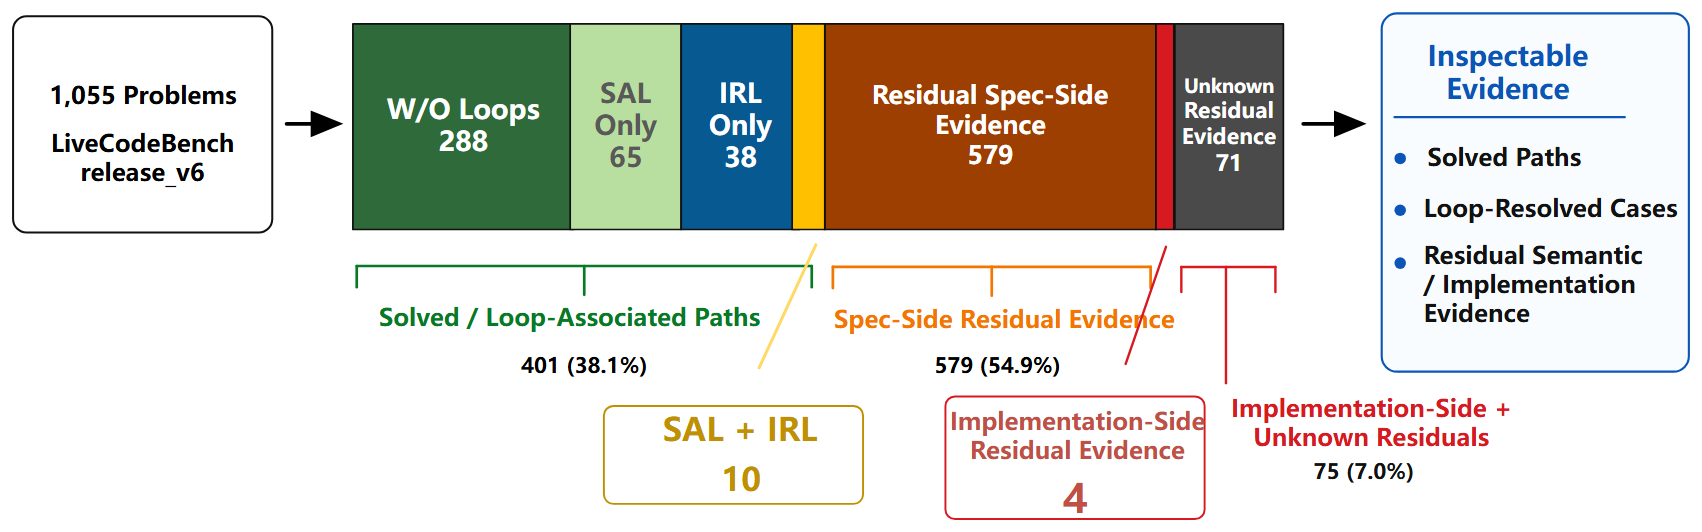
\includegraphics[width=\linewidth]{pics/trace_evidence_cn.png}
\caption{Final-aligned trace evidence.}
\label{fig:trace}
\end{figure}

Figure~\ref{fig:trace} aligns traces with final outcomes. The 401 solved programs comprise 288 paths without loop-associated change, 65 with SAL-associated change, 38 with IRL-associated change, and 10 with both. The remaining traces contain 579 specification-side labels, 4 implementation-side labels, and 71 unknowns. A balanced 36-sample audit obtains 58.3\% strict and 61.1\% relaxed agreement; Appendix~\ref{app:trace-audit} gives the detailed calibration.

\noindent\textit{Answer to RQ4.}
The trace exposes semantic and implementation evidence absent from direct generation, but it supports rather than replaces human analysis.

Together, the results support observable, reusable semantic contracts: SAL exposes semantic-state movement and IRL records verifier-level progress.


\section{Conclusion}

This paper presents a dual-loop NL-to-code framework that makes task semantics explicit before implementation and keeps the accepted contract fixed during verifier-guided repair. On 1,055 LiveCodeBench release\_v6 problems it reaches 0.3801 Final Pass Rate, 3.98 points above the strongest shared-protocol external baseline, while keeping semantic and implementation transitions separately inspectable. The main limits are that the contract is LLM-induced rather than verified, that SAS is a directional signal produced by the same backbone, that trace labels agree with human review only 58.3\% of the time, and that the reported rates are single-run point estimates. Future work will study independent specification review, confidence-aware attribution, broader settings, and budget-normalized activation.

\section*{Ethics Statement}

This work evaluates program synthesis on public competitive-programming benchmarks and involves no human subjects, personal data, or deployment to end users. The only human annotation is the authors' own audit of 36 traces. All generated programs are executed in a sandboxed harness with fixed time limits. The system reports inspectable evidence, not verified correctness: a frozen contract and a satisfied property clause constrain an implementation without proving it correct, and presenting either as a guarantee would be a misuse of the method.

\section*{Reproducibility Statement}

The Experiments section describes the benchmark partitions, feedback restrictions, model, candidate budgets, stopping conditions, and evaluation metric. The appendices provide the complete acceptance predicates, controlled-method definitions, hyperparameter sensitivity results, and additional ablations. Anonymous supplementary code contains the core SAL and IRL procedures, evaluation scripts, configuration fields, and commands needed to reproduce the reported protocol. Private tests are queried only after final program selection.

\section*{AI Use Statement}

Generative AI tools were used to assist with literature discovery, language and formatting checks, and limited manuscript polishing and code editing. All cited sources, implementations, experimental results, and final claims were independently reviewed and verified by the authors, who take full responsibility for the paper.

\bibliography{references}
\bibliographystyle{iclr2027_conference}

\appendix

\section{Complete SAL Acceptance Predicates}
\label{app:gate}

Let $u^{(t)}$, $m^{(t)}$, and $b^{(t)}$ be the numbers of unsupported, missing, and blocking issues returned by the judge; let $c^{(t)}$ be judge confidence, $d^{(t)}$ the number of material semantic items, and $\rho^{(t)}$ aggregate issue pressure. Hatted quantities refer to candidate $\hat{s}^{(t+1)}$. $\mathrm{Valid}^{(t+1)}$ requires a parseable candidate and score record, a patch confined to target fields and disjoint from protected fields, and at least one material semantic change. The complete non-regression predicate is
\begin{align}
\mathrm{Safe}^{(t+1)}\Longleftrightarrow{}&
\mathrm{Valid}^{(t+1)}
\land \mathrm{SAS}(x,\hat{s}^{(t+1)})\geq\mathrm{SAS}^{(t)}
\land \hat q_{\mathrm{faith}}^{(t+1)}\geq q_{\mathrm{faith}}^{(t)}
\land \hat u^{(t+1)}\leq u^{(t)} \nonumber\\
&\land\bigl(\hat m^{(t+1)}\leq m^{(t)}
\lor \hat q_{\mathrm{cov}}^{(t+1)}>q_{\mathrm{cov}}^{(t)}\bigr) \nonumber\\
&\land\bigl(c^{(t)}=0\lor\hat c^{(t+1)}=0
\lor\hat c^{(t+1)}\geq c^{(t)}-10\bigr).
\label{eq:safe-full}
\end{align}
The grounded-progress predicate is
\begin{align}
\mathrm{Improve}^{(t+1)}\Longleftrightarrow{}&
\bigl(\mathrm{SAS}(x,\hat{s}^{(t+1)})-\mathrm{SAS}^{(t)}\geq\delta
\land\rho^{(t)}>0\bigr) \nonumber\\
&\lor(\hat u^{(t+1)}<u^{(t)})
\lor(\hat\rho^{(t+1)}<\rho^{(t)}) \nonumber\\
&\lor\bigl(\hat q_{\mathrm{prec}}^{(t+1)}>q_{\mathrm{prec}}^{(t)}
\land\hat q_{\mathrm{cov}}^{(t+1)}\geq q_{\mathrm{cov}}^{(t)}
\land\rho^{(t)}>0\bigr) \nonumber\\
&\lor\bigl(\hat m^{(t+1)}<m^{(t)}
\land\hat q_{\mathrm{cov}}^{(t+1)}\geq q_{\mathrm{cov}}^{(t)}\bigr) \nonumber\\
&\lor\bigl(\hat b^{(t+1)}<b^{(t)}
\land\hat q_{\mathrm{prec}}^{(t+1)}\geq q_{\mathrm{prec}}^{(t)}\bigr) \nonumber\\
&\lor\bigl(\hat d^{(t+1)}>d^{(t)}
\land\hat q_{\mathrm{prec}}^{(t+1)}>q_{\mathrm{prec}}^{(t)}
\land\rho^{(t)}>0\bigr).
\label{eq:improve-full}
\end{align}
Safety prevents a local revision from damaging already expressed obligations; improvement requires at least one grounded gain. The update in~\eqref{eq:accept} commits the candidate only when both predicates hold.

\section{Additional Experimental Details}
\label{app:additional-results}

\subsection{Compared configurations}

Table~\ref{tab:controlled-methods} records the operational definitions used in the shared evaluation pipeline. Style-matched baselines preserve the feedback form of the cited methods, while the two external adaptations preserve their central workflows under the common model, benchmark loader, verifier, and final evaluator.

\begin{table}[h]
\centering
\small
\begin{tabular}{@{}lp{0.68\linewidth}@{}}
\toprule
Configuration & Operational definition \\
\midrule
Direct NL-to-Code & Generate one program directly from $x$ without iterative feedback. \\
Decomposition Only & Induce $s^{(0)}$ and generate code without SAL or IRL. \\
Self-Refine-style & Execute public tests and iteratively revise code from feedback \citep{ref_self_refine}. \\
Reflexion-style & Accumulate public feedback as verbal reflection and repair from that memory \citep{ref_reflexion}. \\
SAL-only & Induce and gate revisions, then freeze the current specification; no IRL. \\
IRL-only & Generate and repair under unrefined $s^{(0)}$; no SAL revision. \\
SpecFix-BM & Cluster behavior from four probe programs and perform at most one requirement repair within an 11-program cap \citep{ref_specfix}. \\
LPW-adapted & Verify and revise a plan on public examples, then hold it fixed during generation and repair within an 11-program cap \citep{ref_planning_driven_programming}. \\
Full Dual-Loop & Freeze $s^\star$, select $C^{(0)}$, and perform contract-conditioned IRL. \\
\bottomrule
\end{tabular}
\caption{Operational definitions of the compared configurations.}
\label{tab:controlled-methods}
\end{table}

\subsection{Intermediate-representation probe}

On an exploratory 50-problem slice, direct generation scores 0.70. Among explicit intermediate representations, spec-to-code scores 0.60, above plan-to-code at 0.56 and pseudocode-to-code at 0.46. Because each representation adds a generation stage and budgets are not matched, this probe does not show that specifications outperform direct prompting. It instead identifies the strongest tested explicit intermediate for the later refinement and property-compilation operations.

\begin{table}[h]
\centering
\small
\begin{tabular}{@{}lr@{}}
\toprule
Method & Final Pass \up \\
\midrule
Direct NL-to-Code & \textbf{0.700} \\
Plan-to-Code & 0.560 \\
Pseudocode-to-Code & 0.460 \\
Spec-to-Code & 0.600 \\
\bottomrule
\end{tabular}
\caption{Intermediate-representation probe on a 50-problem slice.}
\label{tab:validation}
\end{table}

\subsection{Component ablation}

The controlled 50-problem component slice uses three candidates per problem and is distinct from the two-candidate cross-backbone slice. SAL-only and IRL-only both reach 0.64, while Full reaches 0.72. The eight-point composition gain supports complementarity on this slice, but SAL-only being slightly below Decomposition Only prevents a claim of an isolated SAL performance gain.

\begin{table}[h]
\centering
\small
\begin{tabular}{@{}lccc@{}}
\toprule
Method & SAL & IRL & Final Pass \up \\
\midrule
Decomposition Only & no & no & 0.66 \\
SAL-only & yes & no & 0.64 \\
IRL-only & no & yes & 0.64 \\
Full Dual-Loop & yes & yes & \textbf{0.72} \\
\bottomrule
\end{tabular}
\caption{Controlled component ablation on 50 Qwen problems.}
\label{tab:component}
\end{table}

\subsection{SAL hyperparameter sensitivity}
\label{app:sensitivity}

The sweep uses a fixed 50-problem sample with seed 2027, disables IRL, and generates one deterministic code candidate at temperature zero from the specification current when SAL terminates. It varies $r\in\{80,85,90,95\}$ under the paper weights and compares the paper, uniform, coverage-heavy, faithfulness-heavy, and precision-heavy profiles at $r=90$. Only public feedback is available, so the sweep isolates SAL-side sensitivity from implementation repair and multi-candidate selection.

Table~\ref{tab:sensitivity} reports the fixed 50-problem public-feedback slice. Under $\mathbf w=(0.4,0.4,0.2)$, thresholds from 80 through 95 pass the same 20 problems. The final contracts at $r=90$ and $r=95$ are identical on all 50 problems, and $r=85$ differs from $r=90$ on one. Accepted revisions rise from 14 at $r=85$ to 15 at $r=90$ and do not increase at $r=95$, making 90 the first observed point on the local plateau.

\begin{table}[h]
\centering
\small
\begin{tabular}{@{}llrrr@{}}
\toprule
Group & Setting & Public Pass \up & Accepted & Calls \down \\
\midrule
Threshold & $r=80$ & 0.400 & 1 & 5.18 \\
& $r=85$ & 0.400 & 14 & 6.90 \\
& $r=90$ & 0.400 & 15 & 7.24 \\
& $r=95$ & 0.400 & 15 & 7.24 \\
\midrule
Weights & $(0.4,0.4,0.2)$ & 0.400 & 15 & 7.24 \\
& $(0.333,0.333,0.334)$ & 0.420 & 13 & 7.18 \\
& $(0.6,0.2,0.2)$ & 0.400 & 10 & 7.26 \\
& $(0.2,0.6,0.2)$ & 0.400 & 7 & 7.14 \\
& $(0.2,0.2,0.6)$ & 0.400 & 6 & 6.94 \\
\bottomrule
\end{tabular}
\caption{SAL sensitivity on a fixed 50-problem public-feedback slice.}
\label{tab:sensitivity}
\end{table}

The one-problem difference between the paper and uniform weights is descriptive: their 95\% Wilson intervals, $[0.276,0.538]$ and $[0.294,0.558]$, overlap substantially. Changing $\mathbf w$ also changes the SAS scale, so aggregate SAS values are not compared across profiles. The sweep supports local stability rather than a uniquely optimal configuration.

\subsection{Property-clause coverage}

Table~\ref{tab:properties} reports clauses compiled from accepted contracts and violation events observed over verifier failures; one clause may be evaluated repeatedly. Numeric-output clauses are compiled most often, while numeric and ordering obligations produce the largest observed violation counts. Zero violations mean only that no evaluated output triggered the recorded check.

\begin{table}[h]
\centering
\small
\begin{tabular}{@{}lrr@{}}
\toprule
Clause type & Compiled \up & Violations \\
\midrule
\texttt{numeric\_output} & 1101 & 53 \\
\texttt{modulo\_output} & 159 & 0 \\
\texttt{non\_negative} & 152 & 4 \\
\texttt{sorted\_order} & 69 & 22 \\
\texttt{boolean\_output} & 30 & 0 \\
\texttt{same\_length} & 12 & 0 \\
\texttt{same\_multiset} & 6 & 7 \\
\bottomrule
\end{tabular}
\caption{Property-clause coverage on LiveCodeBench release\_v6.}
\label{tab:properties}
\end{table}

\subsection{Requirement-heavy subsets}

Table~\ref{tab:subsets} connects the mechanism analysis to requirement-heavy tasks. Full exceeds direct generation by 7.13--9.77 points on constraint-heavy, format-sensitive, edge-case-heavy, and semantic-heavy subsets and exceeds Reflexion-style repair in every category. The largest gains occur on format- and edge-case-sensitive problems, where explicit protocol and boundary obligations are especially useful. The slices are derived from benchmark metadata and overlap, so one problem can appear in several of them.

\begin{table}[h]
\centering
\small
\begin{tabular}{@{}lrrr@{}}
\toprule
Subset & Direct & Reflexion & Full \up \\
\midrule
Constraint-heavy & 0.1602 & 0.1869 & \textbf{0.2315} \\
Format-sensitive & 0.2512 & 0.2943 & \textbf{0.3481} \\
Edge-case-heavy & 0.3239 & 0.3702 & \textbf{0.4216} \\
Semantic-heavy & 0.2281 & 0.2643 & \textbf{0.3213} \\
\bottomrule
\end{tabular}
\caption{Performance on requirement-heavy LiveCodeBench subsets.}
\label{tab:subsets}
\end{table}

\section{Trace Audit and Case Study}
\label{app:trace-audit}

\subsection{Trace-label audit}

Figure~\ref{fig:trace} reports the final-aligned trace counts. Its path labels identify where recorded state changed, not which loop alone caused the final outcome. A residual specification-side label likewise records semantic evidence such as a weak accepted specification or unresolved obligation, whereas an implementation-side label requires sufficiently clear contract and verifier evidence.

A balanced 36-sample audit evaluates this distinction (Table~\ref{tab:audit}). It contains 12 solved and 12 system-labeled spec-side samples, together with 12 implementation-side samples supplemented from auxiliary ablations because only four such residual labels appear in the full final-aligned run. The reviewer examines the raw task, accepted specification, final code, latest verifier signal, and system label. Strict agreement is 58.3\% (21 of 36), with one additional partial match for 61.1\% relaxed agreement. The accepted specification is judged fully adequate in 25 cases and partially adequate in 7 more, yielding 88.9\% combined adequacy.

\begin{table}[t]
\centering
\small
\begin{tabular}{@{}lrrrr@{}}
\toprule
Trace label & $n$ & Agree \up & Partial & Disagree \down \\
\midrule
Solved & 12 & 12 & 0 & 0 \\
Spec-side & 12 & 1 & 1 & 10 \\
Impl.-side & 12 & 8 & 0 & 4 \\
Overall & 36 & 21 & 1 & 14 \\
\bottomrule
\end{tabular}
\caption{Human audit of trace-based attribution labels.}
\label{tab:audit}
\end{table}

All 12 solved labels agree with the audit, and 8 of 12 implementation-side labels are confirmed. Spec-side labels are less precise: one is confirmed and one partially matches.

\subsection{Case study}
\label{app:case-study}

\begin{figure}[H]
\centering
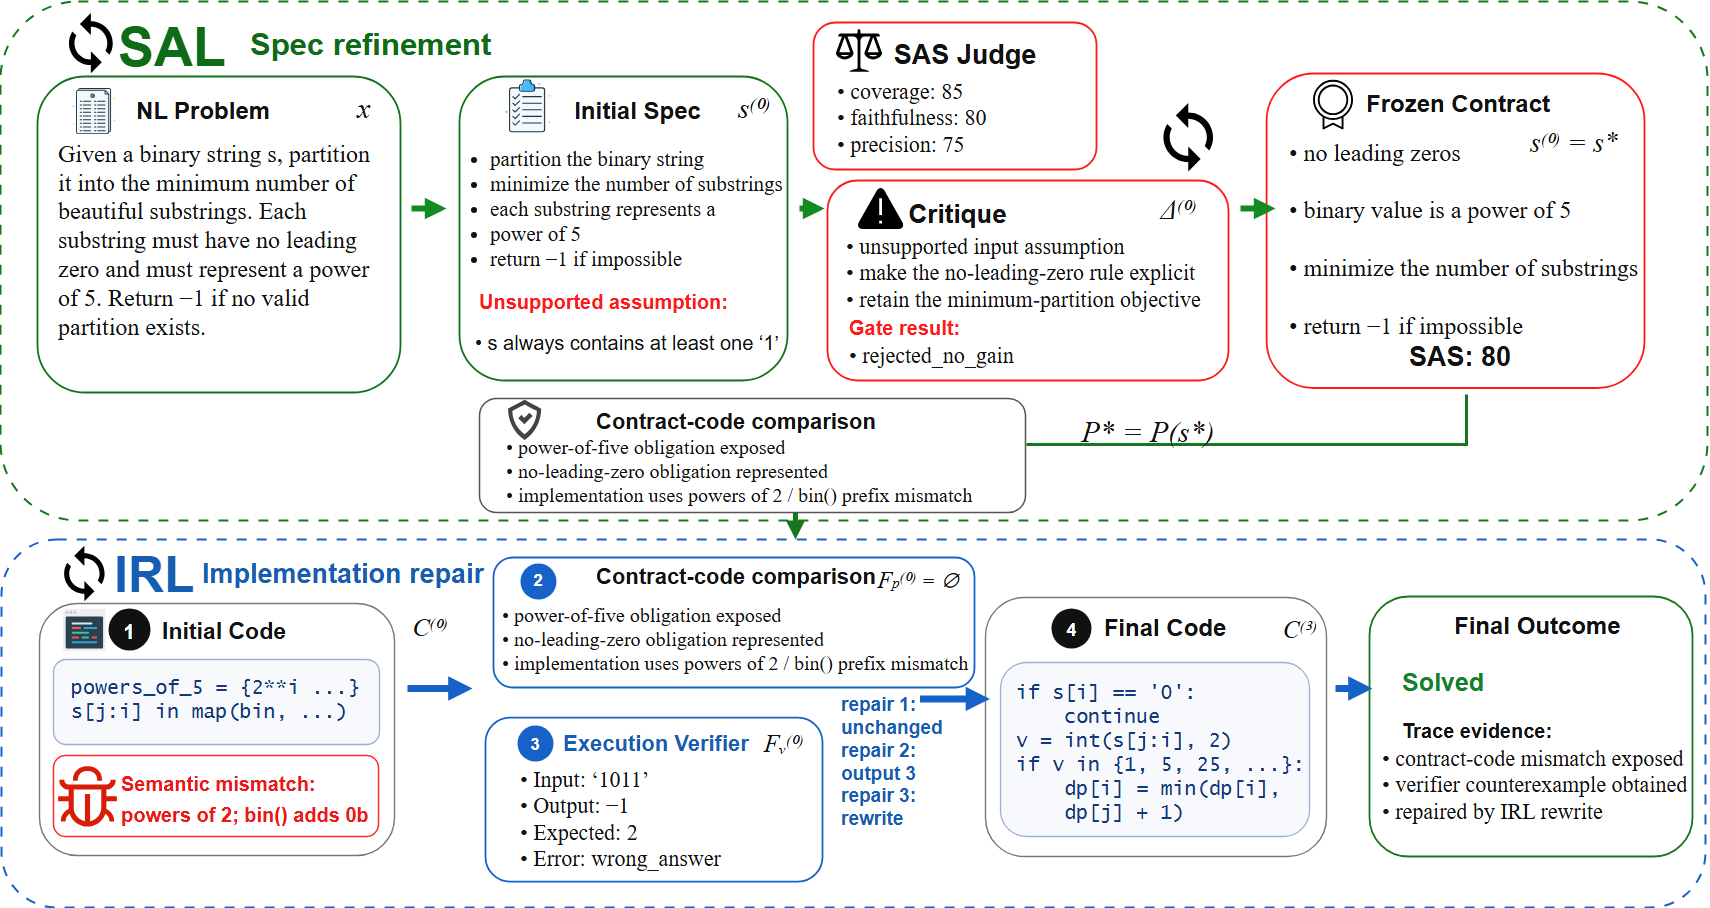
\includegraphics[width=\linewidth]{pics/case_study_cn.png}
\caption{Case-study trace for LiveCodeBench problem 2883.}
\label{fig:case}
\end{figure}

Figure~\ref{fig:case} explains one trace rather than adding an aggregate result. The upper SAL band judges, gates, and freezes the semantic target before implementation, and the lower IRL band checks and repairs code under that target. The task seeks a minimum partition of a binary string into powers of five with no leading zero. Initial $s^{(0)}$ already records the power-of-five condition, no-leading-zero rule, minimum objective, and $-1$ fallback. The judge assigns $q^{(0)}=(85,80,75)$ and, as the aggregate returned under the rubric rather than a recomputed weighted sum, $\mathrm{SAS}^{(0)}=80$; it then proposes a local clarification. Rejudging merged candidate $\hat{s}^{(1)}$ produces no gain, so $\mathrm{Improve}^{(1)}=0$ and the gate rejects it. SAL retains $s^{(0)}$, terminates, and directly freezes that current state: $s^\star=s^{(0)}$ and $\mathrm{SAS}(x,s^\star)=80$. No additional specification variant is generated or selected.

The bridge $P^\star=P(s^\star)$ marks the compiled subset; the contract--code comparison boxes are explanatory, not feedback variables. Initial $C^{(0)}$ constructs powers with \texttt{2**i} and compares substrings with \texttt{bin()} strings retaining the \texttt{0b} prefix.

Feedback $F_v^{(0)}$ exposes the mismatch: for \texttt{"1011"}, the program returns $-1$, while \texttt{"101"}\,$|$\,\texttt{"1"} gives 2. IRL converts substrings with \texttt{int(substring,2)}, checks powers-of-five membership, enforces no leading zero, and updates the dynamic program. Since $F_p^{(0)}=\emptyset$, verifier-guided repair receives credit for this transition. The contract makes the obligation legible; $F_v$ drives the correction.


\end{document}
